\newpage
\section{Projektowanie}		%3

W niniejszym rozdziale przedstawimy szczegółowy opis narzędzi i technologii, które zostały wykorzystane do realizacji projektu, a także opis procesu projektowego.

\subsection{Narzędzia i technologie}

Do stworzenia projektu użyte zostały następujące technologie i narzędzia:

\begin{itemize}
	\item \textbf{Język programowania:} C++ - Został wybrany jako główny język programowania ze względu na jego wydajność oraz obsługę struktur danych, takich jak drzewa.
	\item \textbf{Kompilator:} GCC oraz MINGW-w64 (MSYS2) - Kompilator C++ do kompilacji programu na systemy Linux oraz Windows. W systemie Linux wykorzystywana jest wersja GCC, a w systemie Windows wersja MINGW-w64.
	\item \textbf{System budowania:} CMake oraz Ninja - CMake służy jako system generowania plików Makefile, podczas gdy Ninja jest używane do budowania projektu w sposób szybszy i bardziej efektywny.
	\item \textbf{Kontrola wersji:} Git - Git jest używany do zarządzania kodem źródłowym oraz współpracy w zespole. Repozytorium znajduje się na platformie GitHub.
	\item \textbf{Automatyczna dokumentacja:} Doxygen - Służy do generowania dokumentacji automatycznej z kodu źródłowego.
	\item \textbf{Dokumentacja ręczna:} LaTeX - Dokumentacja projektu jest tworzona przy użyciu szablonu LaTeX dostosowanego przez mgr inż. Dawida Kotlarskiego.
	\item \textbf{Automatyczne testowanie i integracja:} GitHub Actions - Używane do automatycznego testowania oraz integracji kodu. Zawiera również mechanizmy Continuous Integration.
	\item \textbf{Weryfikacja commitów:} Commitlint - Narzędzie do walidacji wiadomości commitów zgodnych z konwencją \textit{Conventional Commits}.
\end{itemize}

\subsection{Konfiguracja kompilatora i środowiska}

Projekt jest skonfigurowany do kompilacji zarówno na systemach Linux jak i Windows. Aby móc efektywnie pracować w obydwu środowiskach, zastosowane zostały odpowiednie konfiguracje:

\begin{itemize}
	\item \textbf{Kompilacja dla Linux (GCC):} Konfiguracja CMake generuje pliki Makefile, które są następnie używane przez GCC w systemie Linux. Kompilacja odbywa się za pomocą polecenia \texttt{make}, co pozwala na szybkie generowanie plików wykonywalnych.
	\item \textbf{Kompilacja dla Windows (MINGW-w64):} Aby umożliwić kompilację w systemie Windows, używamy wersji MINGW-w64 w połączeniu z MSYS2, które zapewnia środowisko linuksowe w systemie Windows. Kompilacja odbywa się przy użyciu polecenia \texttt{mingw32-make}.
\end{itemize}

\subsection{Struktura projektu}

Struktura katalogów projektu jest następująca:

\begin{itemize}
	\item \texttt{src/} - Główny katalog zawierający kod źródłowy.
	\item \texttt{include/} - Katalog z plikami nagłówkowymi.
	\item \texttt{docs/} - Katalog z dokumentacją wygenerowaną przez Doxygen oraz LaTeX.
	\item \texttt{build/} - Katalog używany do przechowywania plików generowanych przez system budowania (np. pliki obiektowe, pliki wykonywalne).
	\item \texttt{tests/} - Katalog zawierający testy jednostkowe.
\end{itemize}

\subsection{Diagramy i schematy}

% \begin{figure}[h!]
% 	\centering
% 	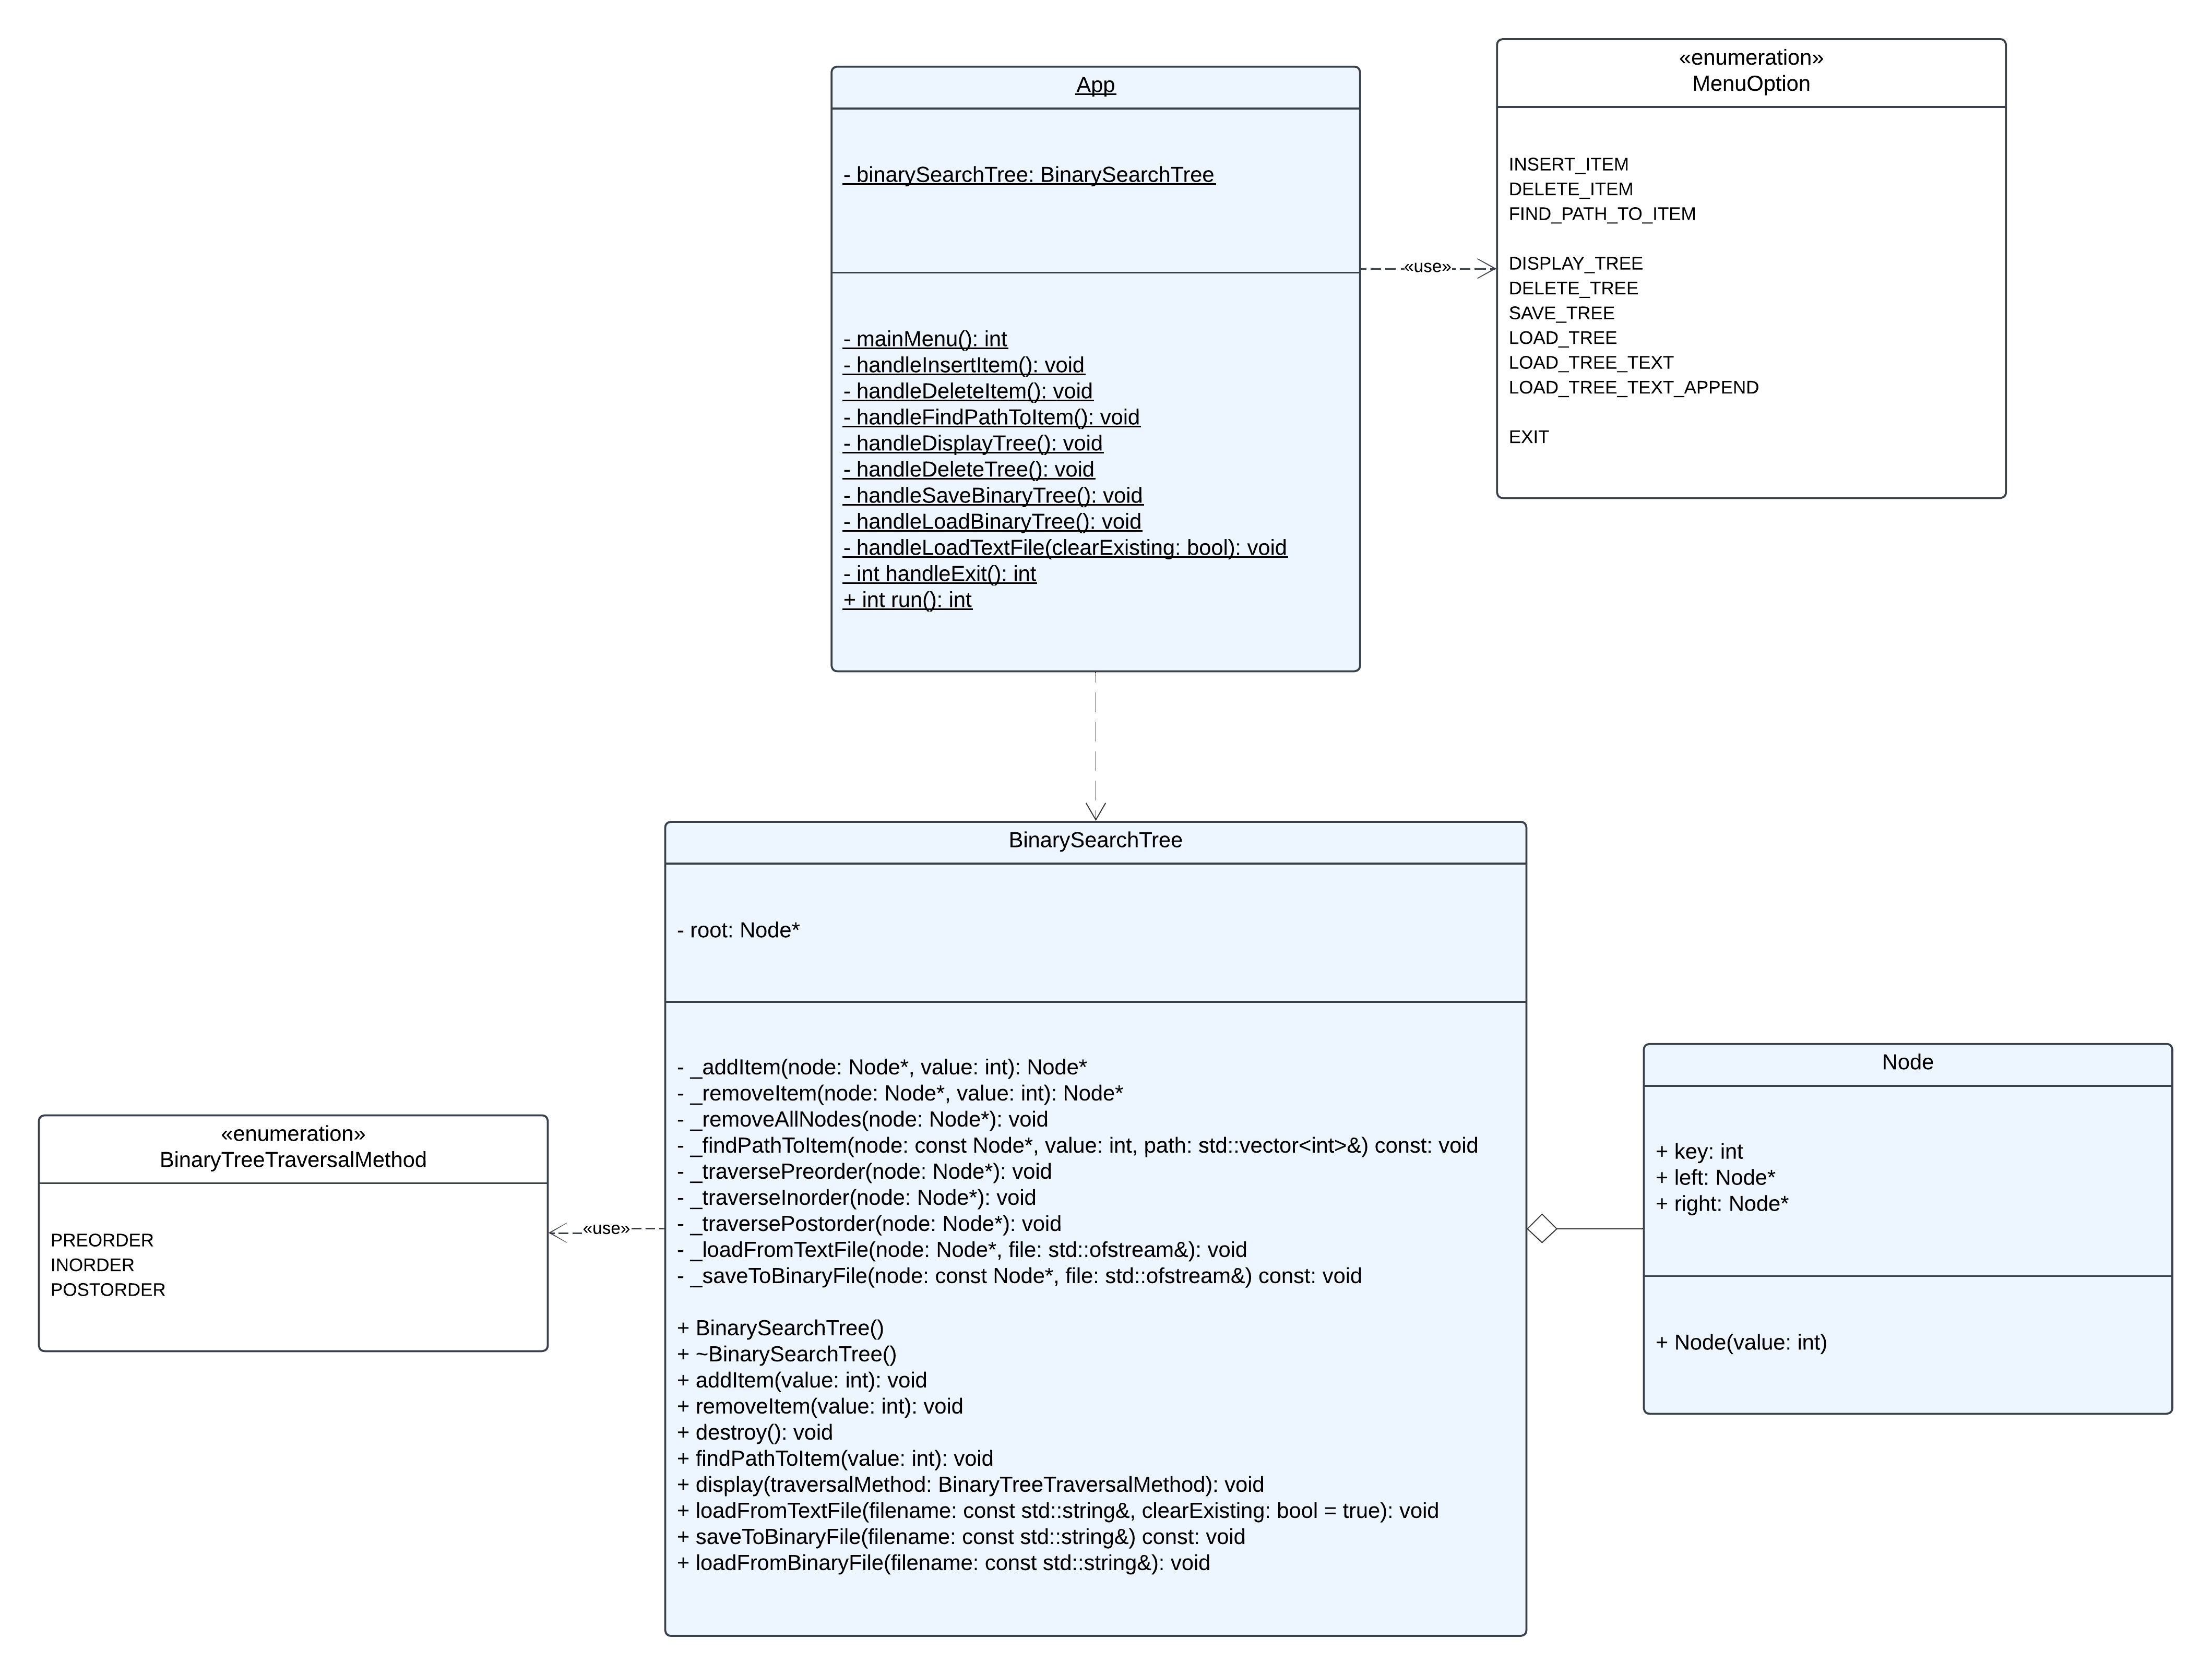
\includegraphics[width=0.8\textwidth]{uml_diagram.png}
% 	\caption{Diagram UML klas aplikacji - pokazuje zależności między klasami BinarySearchTree oraz App.}
% 	\label{fig:uml_diagram}
% \end{figure}

W projekcie zastosowano klasy \texttt{BinarySearchTree} oraz \texttt{App}. Klasa \texttt{BinarySearchTree} odpowiada za przechowywanie struktury drzewa oraz wykonanie operacji na drzewie (dodawanie, usuwanie, przeglądanie). Klasa \texttt{App} zapewnia interfejs użytkownika oraz umożliwia zarządzanie drzewem za pomocą menu.

\begin{itemize}
	\item \textbf{Klasa BinarySearchTree:} Przechowuje dane drzewa oraz implementuje operacje na nim, takie jak dodawanie elementów, usuwanie, przeglądanie w różnych metodach (preorder, inorder, postorder).
	\item \textbf{Klasa App:} Zapewnia menu, które umożliwia użytkownikowi interakcję z drzewem: dodawanie, usuwanie elementów oraz wyświetlanie struktury drzewa.
\end{itemize}

\subsection{Git i narzędzia CI/CD}

Projekt oparty jest na systemie kontroli wersji Git, z repozytorium umieszczonym na platformie GitHub. GitHub Actions jest wykorzystywane do automatyzacji procesu budowania i testowania projektu. Do weryfikacji wiadomości commitów stosowana jest konwencja \textit{Conventional Commits} i narzędzie \texttt{Commitlint}.

\subsection{Przykład użycia Git}

Poniżej przedstawiono przykładową procedurę pracy z projektem przy użyciu Git:

\begin{itemize}
	\item \textbf{Tworzenie nowego brancha:} Aby rozpocząć pracę nad nową funkcjonalnością, użytkownik tworzy nowy branch:
	      \begin{verbatim}
    git checkout -b feature-new-feature
    \end{verbatim}
	\item \textbf{Dodawanie zmian:} Po wprowadzeniu zmian, użytkownik dodaje je do systemu kontroli wersji:
	      \begin{verbatim}
    git add .
    \end{verbatim}
	\item \textbf{Commit zmian:} Następnie użytkownik wykonuje commit:
	      \begin{verbatim}
    git commit -m "feat: dodanie nowej funkcjonalności"
    \end{verbatim}
	\item \textbf{Wysyłanie zmian na GitHub:} Po wykonaniu kilku commitów, użytkownik wysyła zmiany do repozytorium:
	      \begin{verbatim}
    git push origin feature-new-feature
    \end{verbatim}
	\item \textbf{Scalanie zmian:} Po zakończeniu pracy nad funkcjonalnością, branch jest scalany do głównego brancha (np. \texttt{main}):
	      \begin{verbatim}
    git checkout main
    git pull origin main
    git merge feature-new-feature
    git push origin main
    \end{verbatim}
\end{itemize}

\subsection{Podsumowanie}

W projekcie wykorzystano szereg narzędzi i technologii, które pozwalają na skuteczną i efektywną pracę nad projektem. Dzięki zastosowaniu systemów takich jak Git oraz GitHub Actions, proces integracji i testowania jest zautomatyzowany, co umożliwia szybkie wykrywanie błędów oraz integrację nowych funkcjonalności. Dokumentacja generowana przez Doxygen oraz LaTeX zapewnia jasny i profesjonalny sposób dokumentowania projektu.
